%!TEX root = main.tex
\chapter{Supplementary Results on Lighting Estimation}     % numérotée
\label{annex3}

\DeclareGraphicsExtensions{.pdf,.jpeg,.png,.jpg}
\graphicspath{{annex3_figures/}}


In this annex, we first provide in table~\ref{tab:sun-visibility} the mean sun visibility (in \%) for all day in the database. We also provide results for all days in the database for: 
\vspace{-.5em}
\paragraph{Fig.~\ref{fig:events} from chapter~\ref{ch1}} Fine-grained analysis of the expected uncertainty of outdoor PS. See results for all days in figs~\ref{fig:fig-5-1} and \ref{fig:fig-5-2}.


\paragraph{Fig.~\ref{fig:ratios} from chapter~\ref{ch1}} Distribution of noise gain ratio $r_t$ as a function of time interval duration. See results for all days in figs~\ref{fig:fig-6-1} and \ref{fig:fig-6-2}.

\vspace{1em}


We also provide reconstruction results for an owl statuette and a bunny model on November 6th, 2013. Reconstruction is performed on images such as the one shown in fig.~\ref{fig:luxrender-input}. These images were obtained using the physically-based renderer LuxRender. For each image, one environment map from the database capturing the whole sky in HDR was used as the sole light source. In each environment map was added an infinite plane on the ground, obtained by simulating asphalt with an albedo $\rho = 0.15$ from which the whole sky is visible. The number of input images for each interval is shown in table~\ref{tab:luxrender-qty-input}. Reconstruction results are shown in fig.~\ref{fig:luxrender-results}. For information on the reconstruction algorithm or more results on synthetic and real data, please refer to the paper.


\begin{table}[!h]
\centering
\begin{tabular}{c|c}
Day & Sun visibility (\%) \\
\hline
11-JUL-13 & 34  \\
08-AUG-13 & 66  \\
23-AUG-13 & 66  \\
24-AUG-13 & 83  \\
06-NOV-13 & 41  \\
11-NOV-13 & 3   \\
15-NOV-13 & 62  \\
19-NOV-13 & 0   \\
03-OCT-14 & 81  \\
06-OCT-14 & 33  \\
11-OCT-14 & 52  \\
20-OCT-14 & 46  \\
21-OCT-14 & 21  \\
22-OCT-14 & 71  \\
30-OCT-14 & 61  \\
02-NOV-14 & 31  \\
03-NOV-14 & 73  \\
06-NOV-14 & 22  \\
08-NOV-14 & 19  \\
10-NOV-14 & 53  \\
11-NOV-14 & 61  \\ 
13-NOV-14 & 55  \\
14-NOV-14 & 55
\end{tabular}
\vspace{.5em}
\caption{Mean sun visibility (in \%) for all days in the database. Sun visibility denotes the fraction of the time the sun is shining, as computed from its intensity in the light probe.}
\label{tab:sun-visibility}
\end{table}


\newlength{\mylength}
\setlength{\mylength}{.31\linewidth}
\newlength{\eventswidth}
\setlength{\eventswidth}{.23\linewidth}
\newlength{\sunintwidth}
\setlength{\sunintwidth}{.04\linewidth}
\newlength{\eventheight}
\setlength{\eventheight}{109pt}
%\setlength{\eventheight}{119pt}
%\setlength{\eventheight}{132pt}
\newlength{\colorbarwidth}
\setlength{\colorbarwidth}{.02\linewidth}

\begin{figure*}
\centering
\begin{minipage}[c]{\mylength}
\centering \scriptsize 11-JUL-13 \\
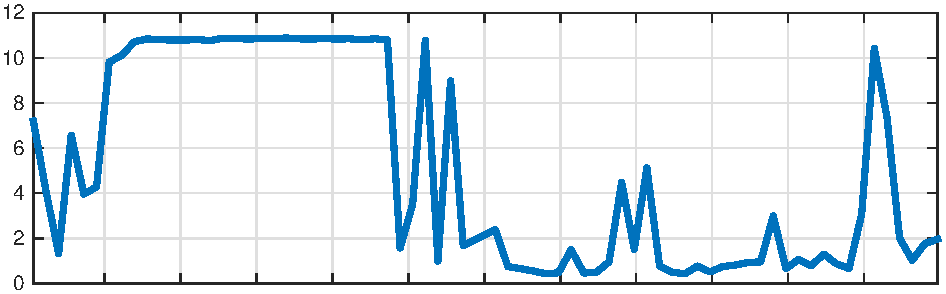
\includegraphics[valign=t,trim=0 0 5pt 0,angle=90,origin=tr,width=\sunintwidth,totalheight=\eventheight]{events/20130711-intensity.pdf}
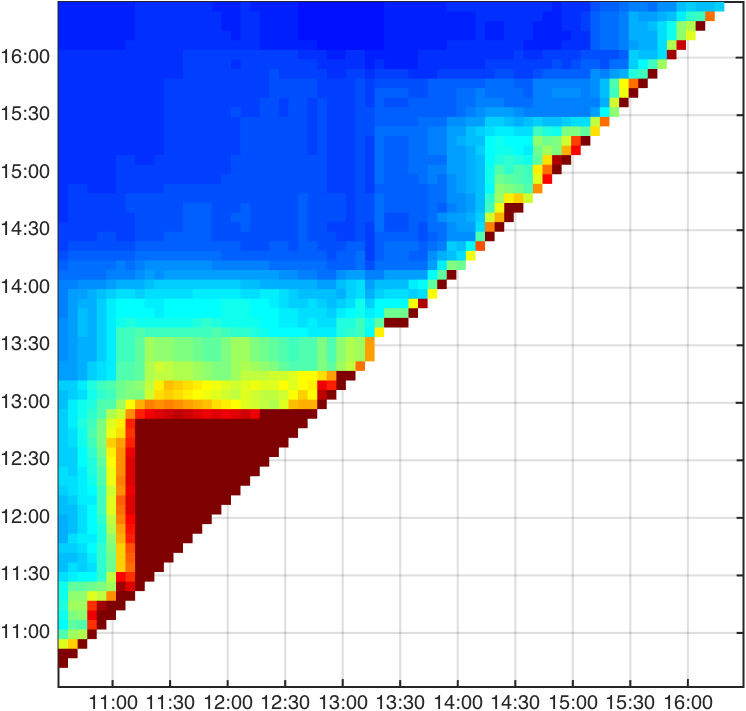
\includegraphics[valign=t,width=\eventswidth]{events/20130711-maxGain-local-events.png}
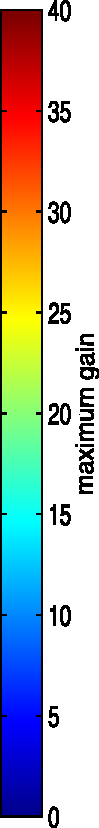
\includegraphics[valign=t,trim=2pt -8pt 0 5pt,trim=2pt -8pt 0 5pt,width=\colorbarwidth,totalheight=\eventheight]{events/colorbar-40.pdf}
\end{minipage}
\begin{minipage}[c]{\mylength}
\centering \scriptsize 16-AUG-13 \\
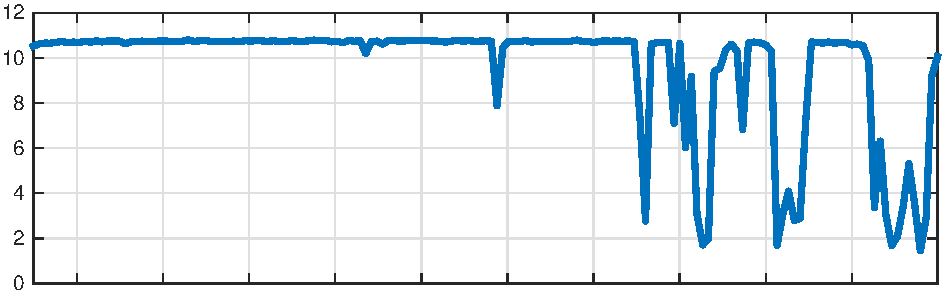
\includegraphics[valign=t,trim=0 0 5pt 0,angle=90,origin=tr,width=\sunintwidth,totalheight=\eventheight]{events/20130816-intensity.pdf}
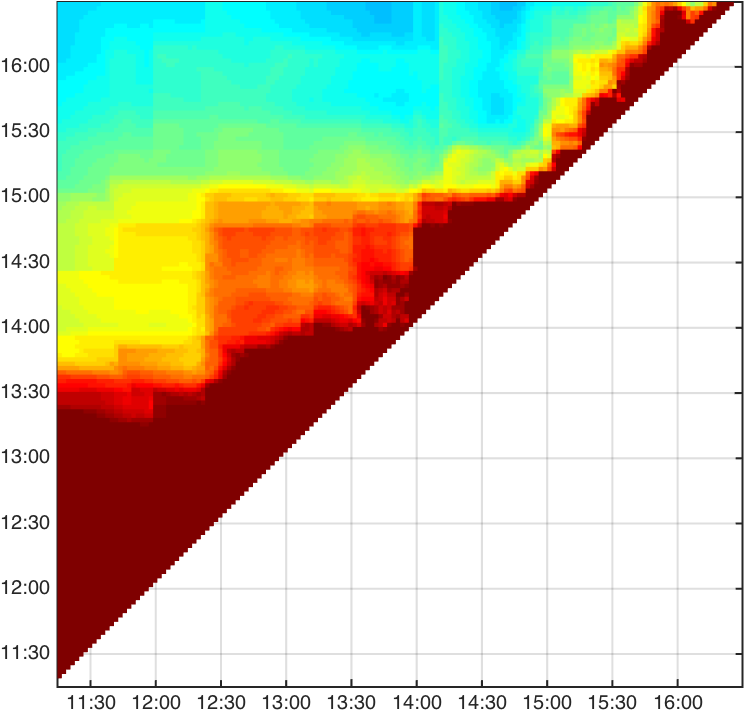
\includegraphics[valign=t,width=\eventswidth]{events/20130816-maxGain-local-events.png}
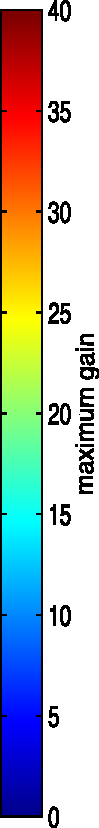
\includegraphics[valign=t,trim=2pt -8pt 0 5pt,width=\colorbarwidth,totalheight=\eventheight]{events/colorbar-40.pdf}
\end{minipage}
\begin{minipage}[c]{\mylength}
\centering \scriptsize 23-AUG-13 \\
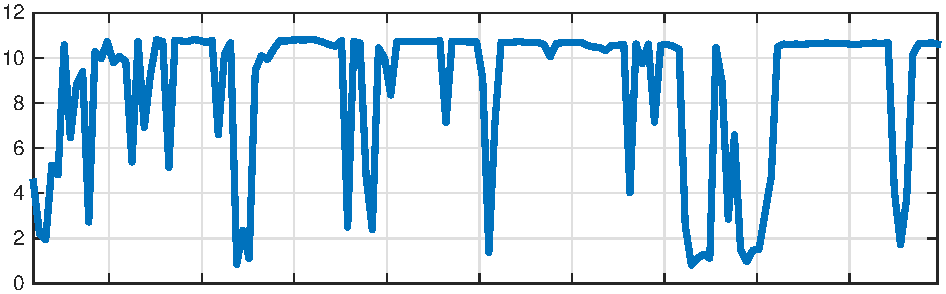
\includegraphics[valign=t,trim=0 0 5pt 0,angle=90,origin=tr,width=\sunintwidth,totalheight=\eventheight]{events/20130823-intensity.pdf}
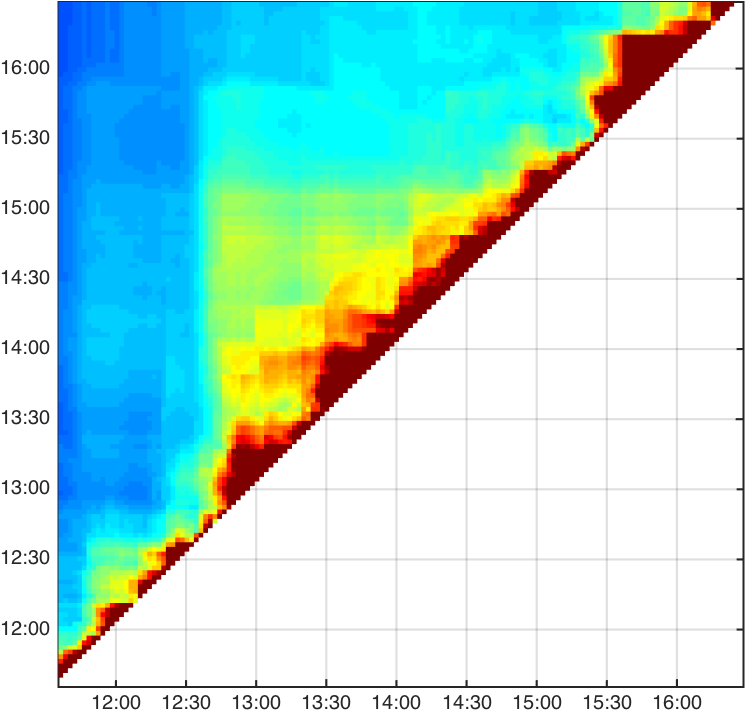
\includegraphics[valign=t,width=\eventswidth]{events/20130823-maxGain-local-events.png}
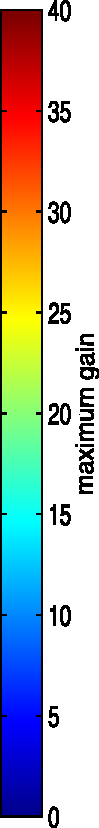
\includegraphics[valign=t,trim=2pt -8pt 0 5pt,width=\colorbarwidth,totalheight=\eventheight]{events/colorbar-40.pdf}
\end{minipage}  \\*[1em]
\begin{minipage}[c]{\mylength}
\centering \scriptsize 24-AUG-13 \\
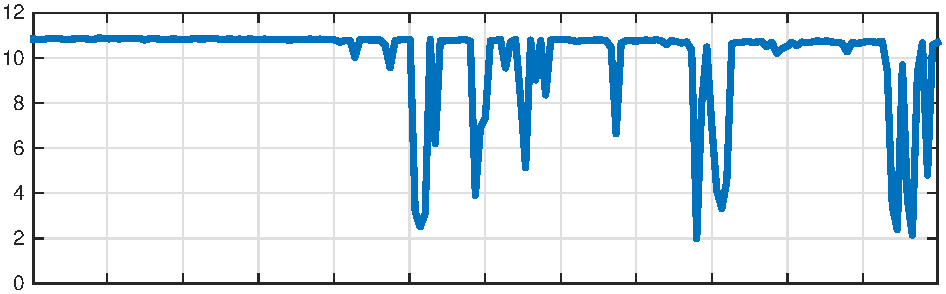
\includegraphics[valign=t,trim=0 0 5pt 0,angle=90,origin=tr,width=\sunintwidth,totalheight=\eventheight]{events/20130824-intensity.pdf}
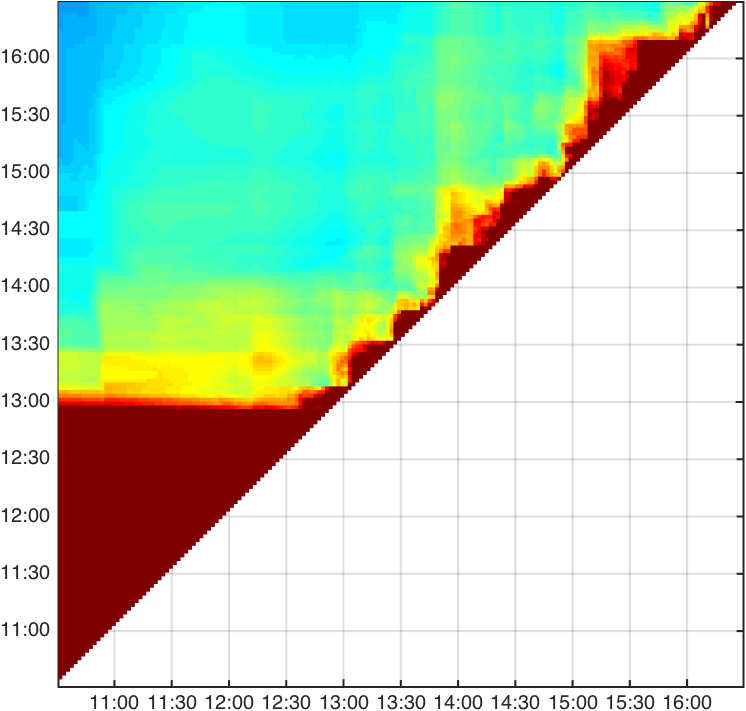
\includegraphics[valign=t,width=\eventswidth]{events/20130824-maxGain-local-events.png}
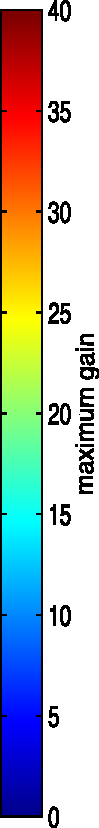
\includegraphics[valign=t,trim=2pt -8pt 0 5pt,width=\colorbarwidth,totalheight=\eventheight]{events/colorbar-40.pdf}
\end{minipage}
\begin{minipage}[c]{\mylength}
\centering \scriptsize 6-NOV-13 \\
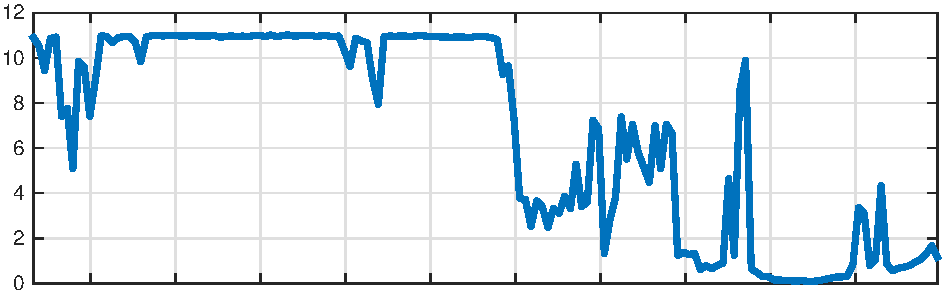
\includegraphics[valign=t,trim=0 0 5pt 0,angle=90,origin=tr,width=\sunintwidth,totalheight=\eventheight]{events/20131106-intensity.pdf}
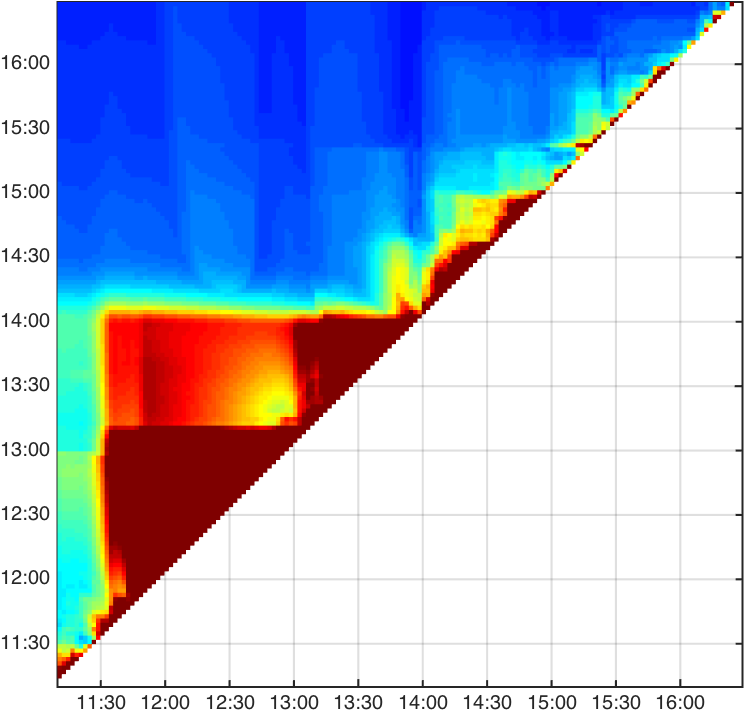
\includegraphics[valign=t,width=\eventswidth]{events/20131106-maxGain-local-events.png}
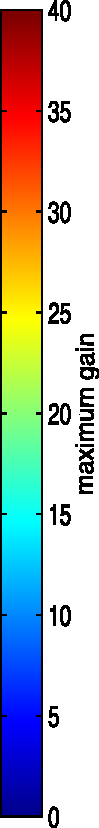
\includegraphics[valign=t,trim=2pt -8pt 0 5pt,width=\colorbarwidth,totalheight=\eventheight]{events/colorbar-40.pdf}
\end{minipage}
\begin{minipage}[c]{\mylength}
\centering \scriptsize 11-NOV-13 \\
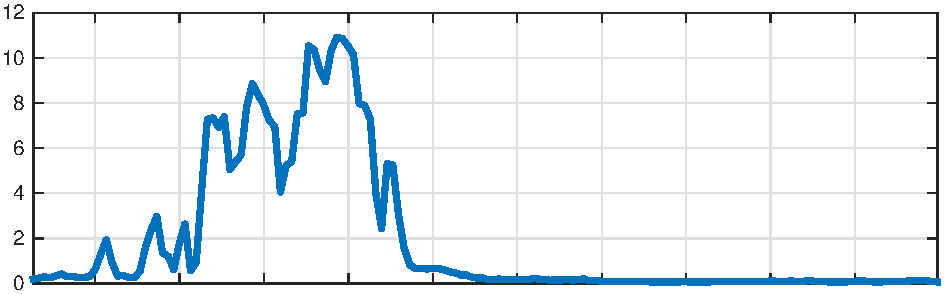
\includegraphics[valign=t,trim=0 0 5pt 0,angle=90,origin=tr,width=\sunintwidth,totalheight=\eventheight]{events/20131111-intensity.pdf}
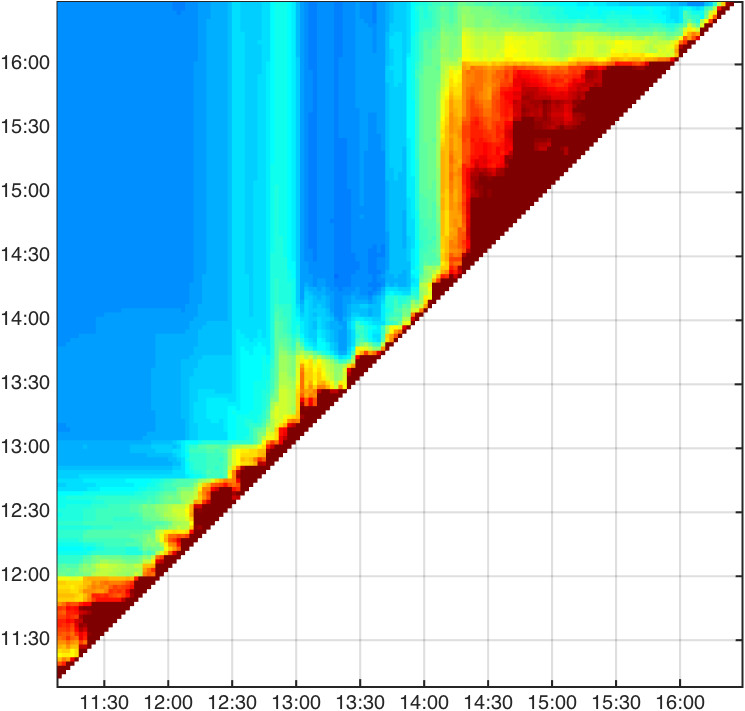
\includegraphics[valign=t,width=\eventswidth]{events/20131111-maxGain-local-events.png}
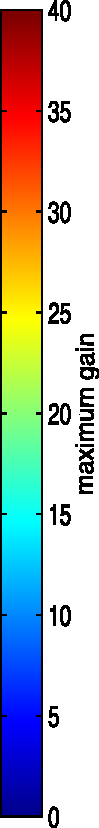
\includegraphics[valign=t,trim=2pt -8pt 0 5pt,width=\colorbarwidth,totalheight=\eventheight]{events/colorbar-40.pdf}
\end{minipage}  \\*[1em]
\begin{minipage}[c]{\mylength}
\centering \scriptsize 15-NOV-13 \\
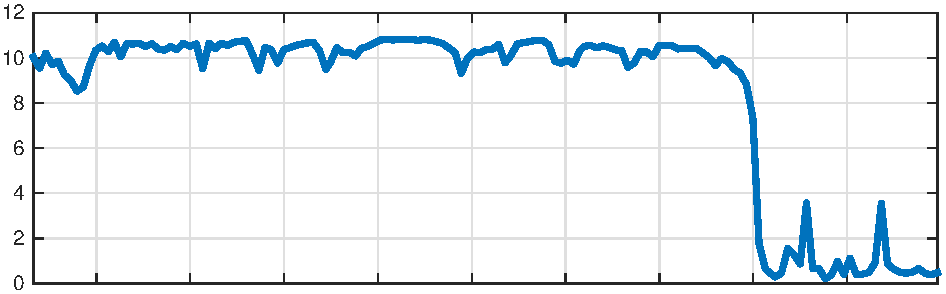
\includegraphics[valign=t,trim=0 0 5pt 0,angle=90,origin=tr,width=\sunintwidth,totalheight=\eventheight]{events/20131115-intensity.pdf}
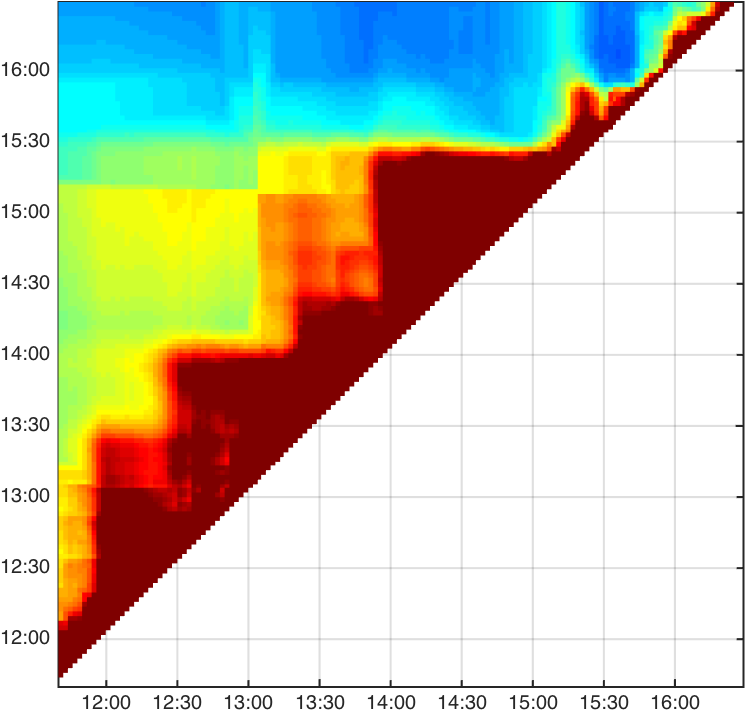
\includegraphics[valign=t,width=\eventswidth]{events/20131115-maxGain-local-events.png}
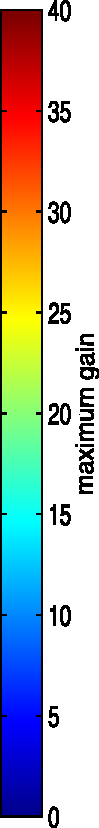
\includegraphics[valign=t,trim=2pt -8pt 0 5pt,width=\colorbarwidth,totalheight=\eventheight]{events/colorbar-40.pdf}
\end{minipage}
\begin{minipage}[c]{\mylength}
\centering \scriptsize 19-NOV-13 \\
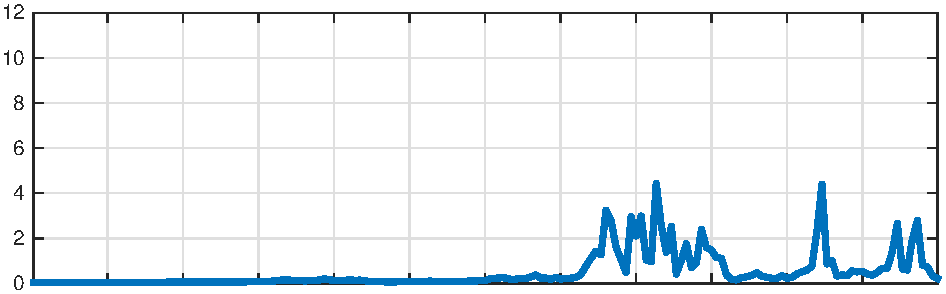
\includegraphics[valign=t,trim=0 0 5pt 0,angle=90,origin=tr,width=\sunintwidth,totalheight=\eventheight]{events/20131119-intensity.pdf}
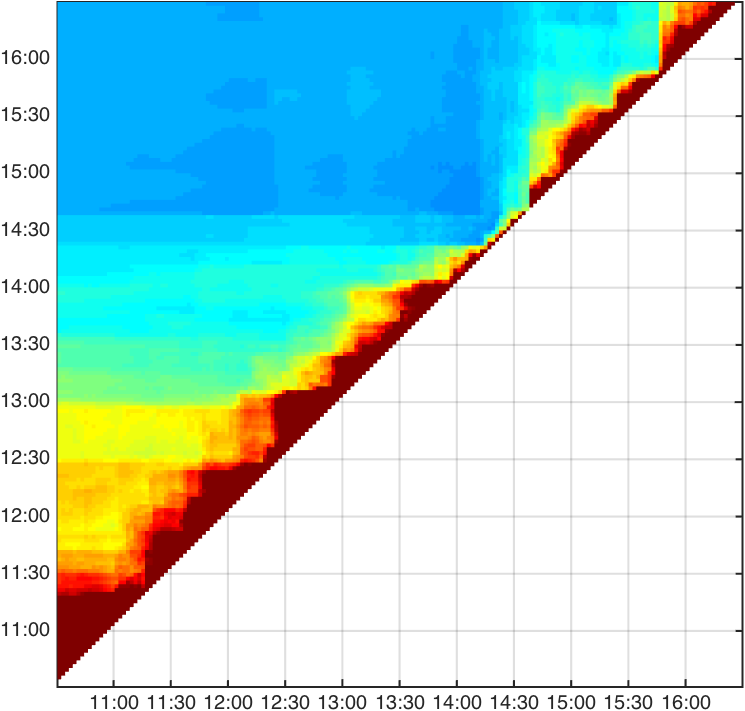
\includegraphics[valign=t,width=\eventswidth]{events/20131119-maxGain-local-events.png}
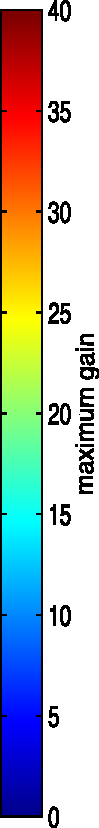
\includegraphics[valign=t,trim=2pt -8pt 0 5pt,width=\colorbarwidth,totalheight=\eventheight]{events/colorbar-40.pdf}
\end{minipage}
\begin{minipage}[c]{\mylength}
\centering \scriptsize 3-OCT-14 \\
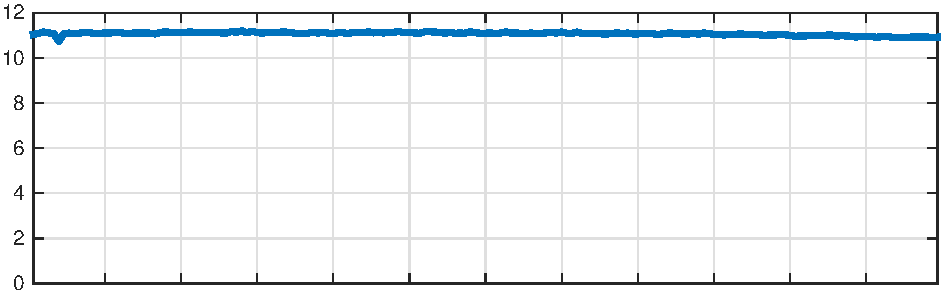
\includegraphics[valign=t,trim=0 0 5pt 0,angle=90,origin=tr,width=\sunintwidth,totalheight=\eventheight]{events/20141003-intensity.pdf}
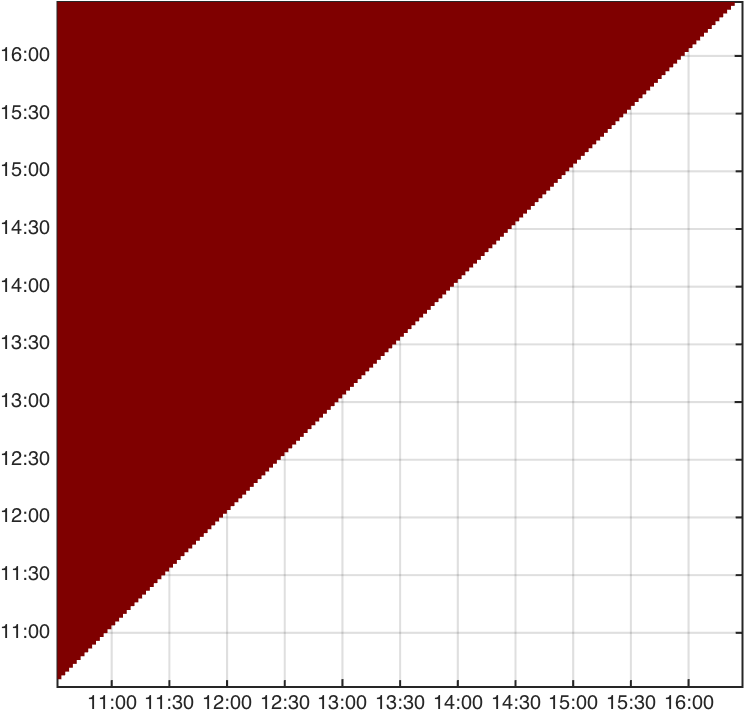
\includegraphics[valign=t,width=\eventswidth]{events/20141003-maxGain-local-events.png}
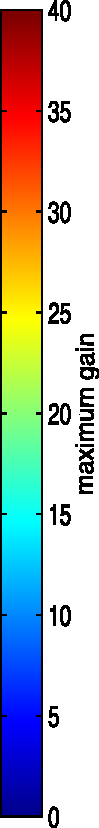
\includegraphics[valign=t,trim=2pt -8pt 0 5pt,width=\colorbarwidth,totalheight=\eventheight]{events/colorbar-40.pdf}
\end{minipage}  \\*[1em]
\begin{minipage}[c]{\mylength}
\centering \scriptsize 6-OCT-14 \\
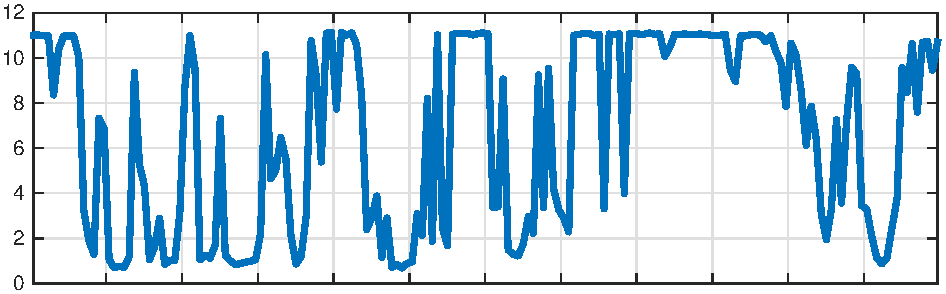
\includegraphics[valign=t,trim=0 0 5pt 0,angle=90,origin=tr,width=\sunintwidth,totalheight=\eventheight]{events/20141006-intensity.pdf}
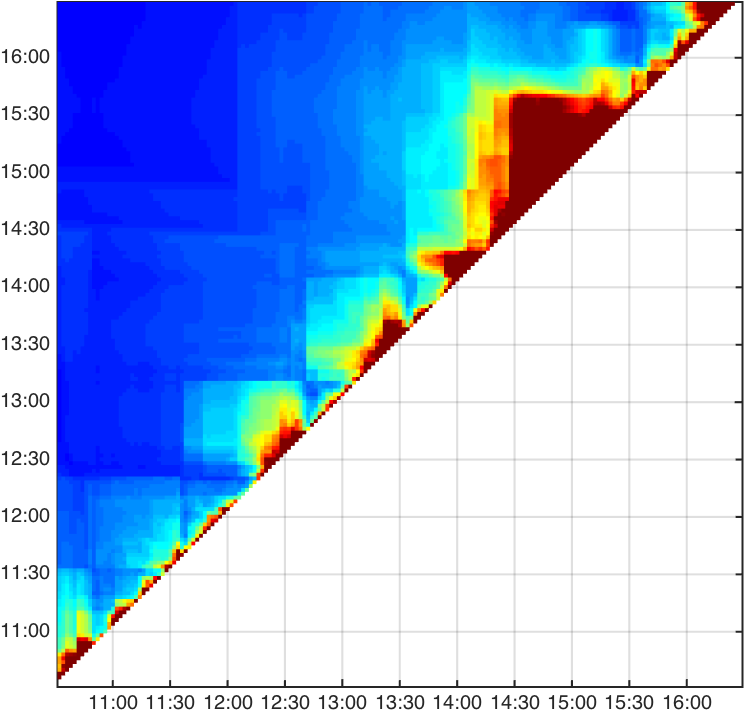
\includegraphics[valign=t,width=\eventswidth]{events/20141006-maxGain-local-events.png}
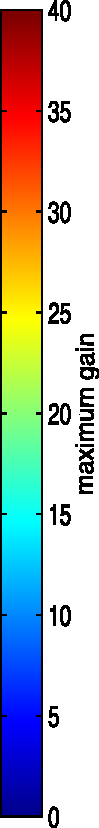
\includegraphics[valign=t,trim=2pt -8pt 0 5pt,width=\colorbarwidth,totalheight=\eventheight]{events/colorbar-40.pdf}
\end{minipage}
\begin{minipage}[c]{\mylength}
\centering \scriptsize 11-OCT-14 \\
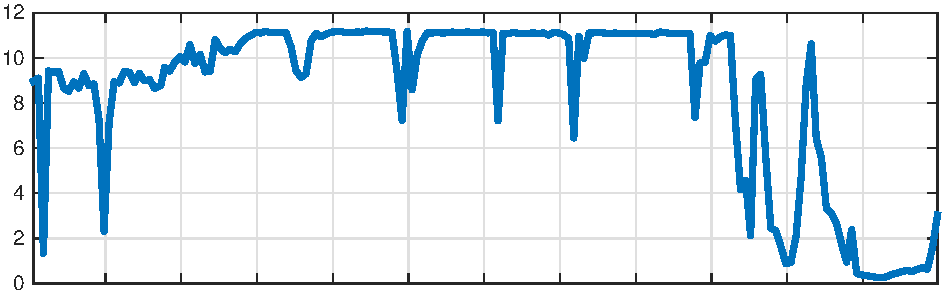
\includegraphics[valign=t,trim=0 0 5pt 0,angle=90,origin=tr,width=\sunintwidth,totalheight=\eventheight]{events/20141011-intensity.pdf}
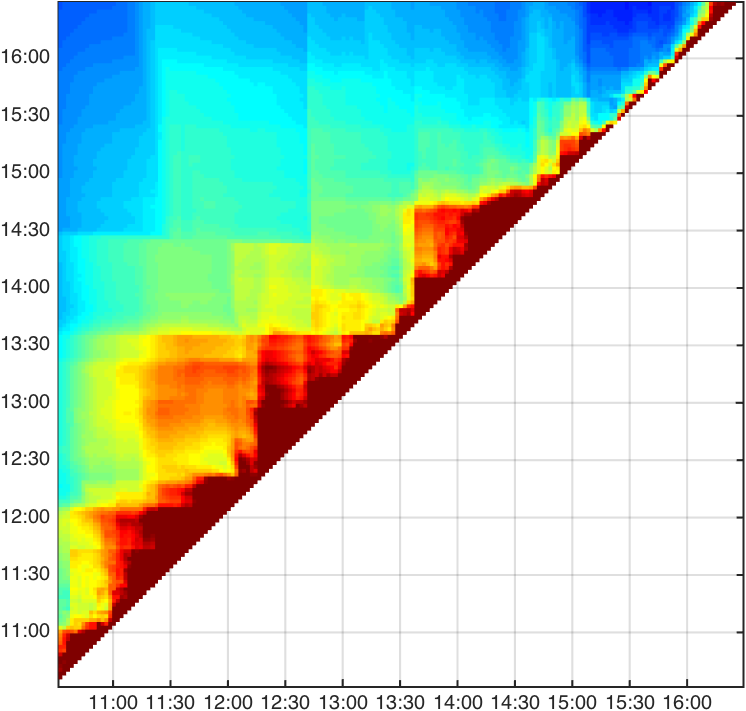
\includegraphics[valign=t,width=\eventswidth]{events/20141011-maxGain-local-events.png}
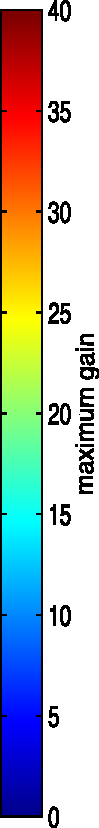
\includegraphics[valign=t,trim=2pt -8pt 0 5pt,width=\colorbarwidth,totalheight=\eventheight]{events/colorbar-40.pdf}
\end{minipage}
\begin{minipage}[c]{\mylength}
\centering \scriptsize 20-OCT-14 \\
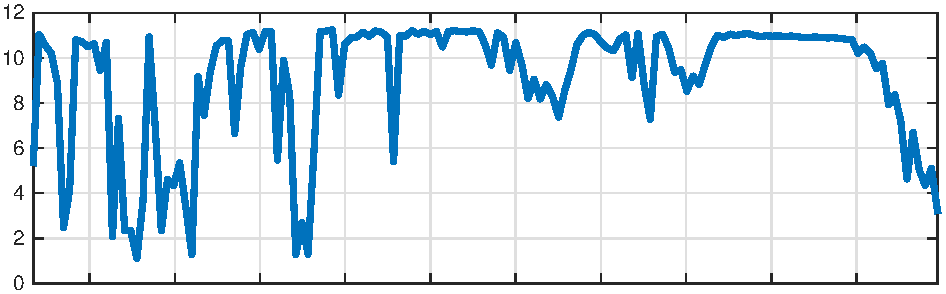
\includegraphics[valign=t,trim=0 0 5pt 0,angle=90,origin=tr,width=\sunintwidth,totalheight=\eventheight]{events/20141020-intensity.pdf}
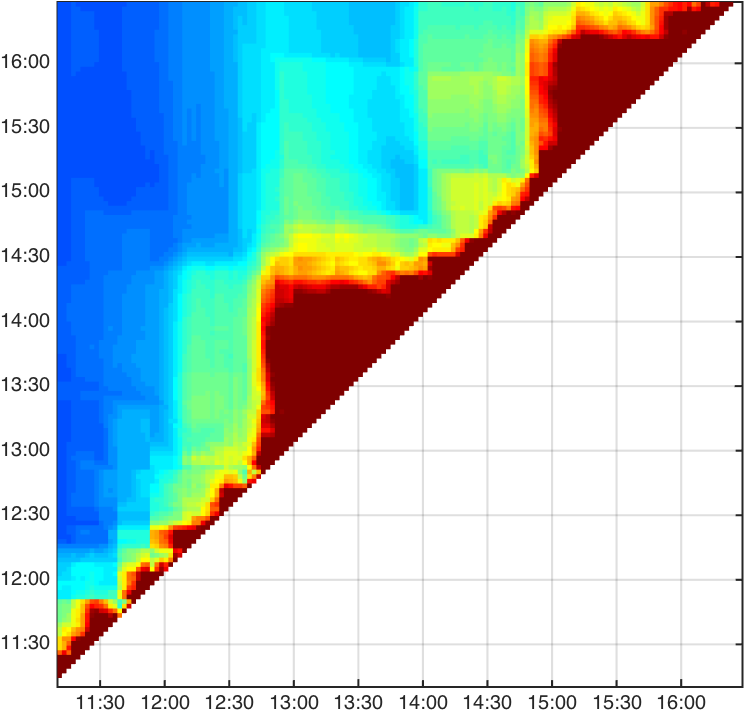
\includegraphics[valign=t,width=\eventswidth]{events/20141020-maxGain-local-events.png}
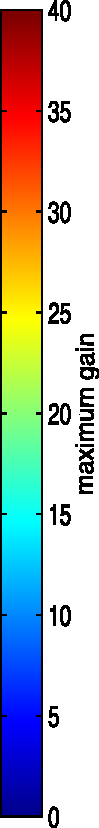
\includegraphics[valign=t,trim=2pt -8pt 0 5pt,width=\colorbarwidth,totalheight=\eventheight]{events/colorbar-40.pdf}
\end{minipage}
\vspace{.5em}
\caption{Fine-grained analysis of the expected uncertainty of outdoor PS (additional results for fig. 5 in the paper). Blank spaces above the diagonal indicate time intervals with missing data. Continued on fig.~\ref{fig:fig-5-2}.}
\label{fig:fig-5-1}
\end{figure*}

\begin{figure*}
\centering
\begin{minipage}[c]{\mylength}
\centering \scriptsize 21-OCT-14 \\
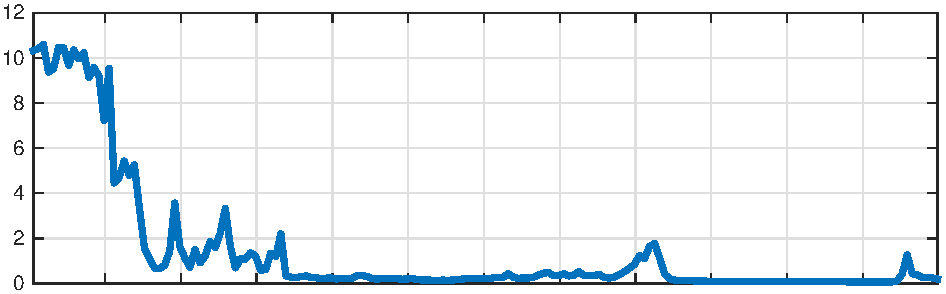
\includegraphics[valign=t,trim=0 0 5pt 0,angle=90,origin=tr,width=\sunintwidth,totalheight=\eventheight]{events/20141021-intensity.pdf}
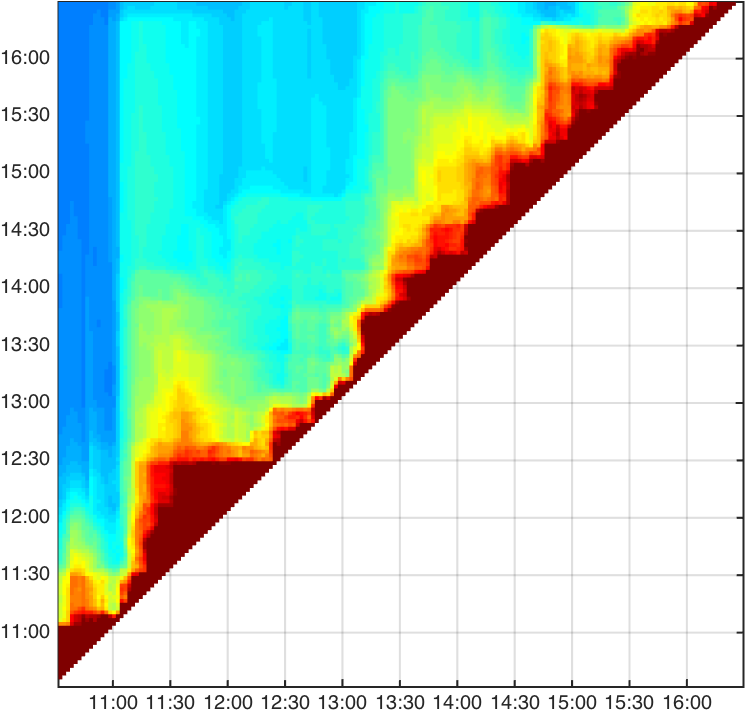
\includegraphics[valign=t,width=\eventswidth]{events/20141021-maxGain-local-events.png}
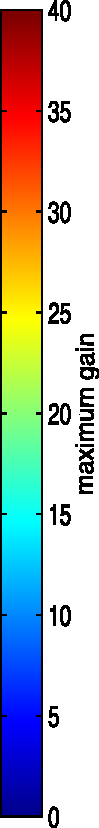
\includegraphics[valign=t,trim=2pt -8pt 0 5pt,width=\colorbarwidth,totalheight=\eventheight]{events/colorbar-40.pdf}
\end{minipage}
\begin{minipage}[c]{\mylength}
\centering \scriptsize 22-OCT-14 \\
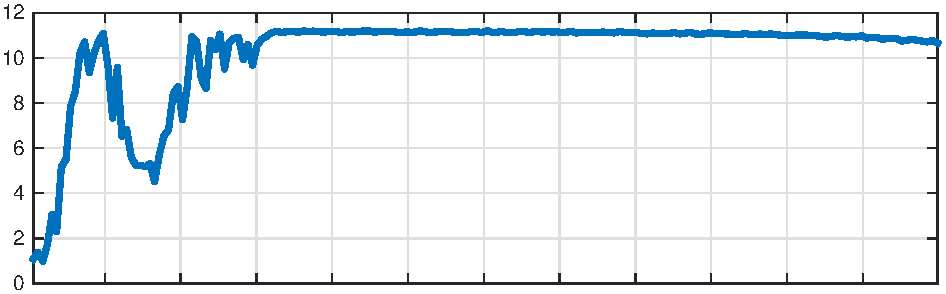
\includegraphics[valign=t,trim=0 0 5pt 0,angle=90,origin=tr,width=\sunintwidth,totalheight=\eventheight]{events/20141022-intensity.pdf}
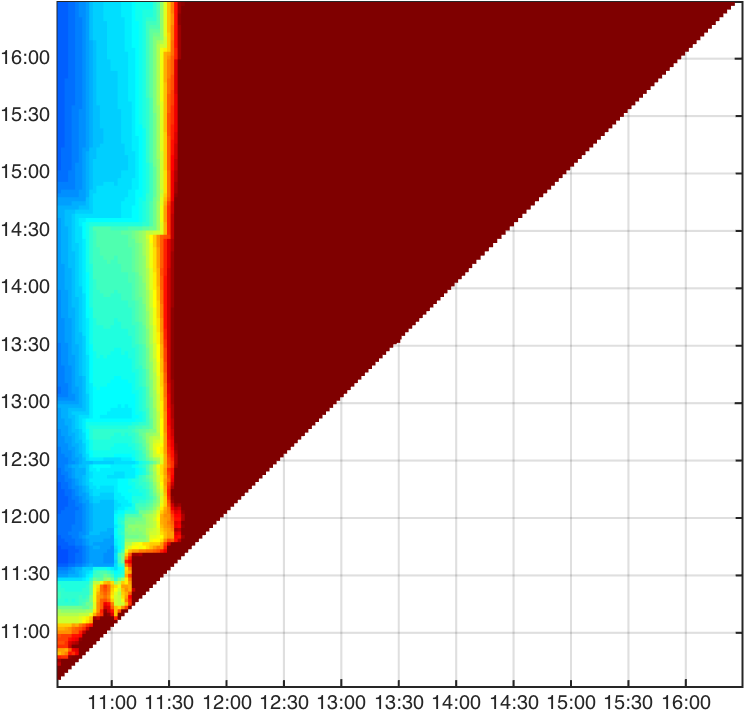
\includegraphics[valign=t,width=\eventswidth]{events/20141022-maxGain-local-events.png}
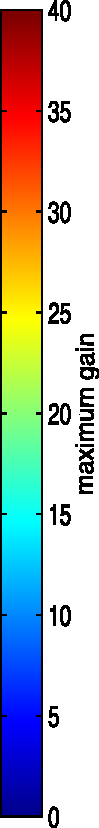
\includegraphics[valign=t,trim=2pt -8pt 0 5pt,width=\colorbarwidth,totalheight=\eventheight]{events/colorbar-40.pdf}
\end{minipage}
\begin{minipage}[c]{\mylength}
\centering \scriptsize 30-OCT-14 \\
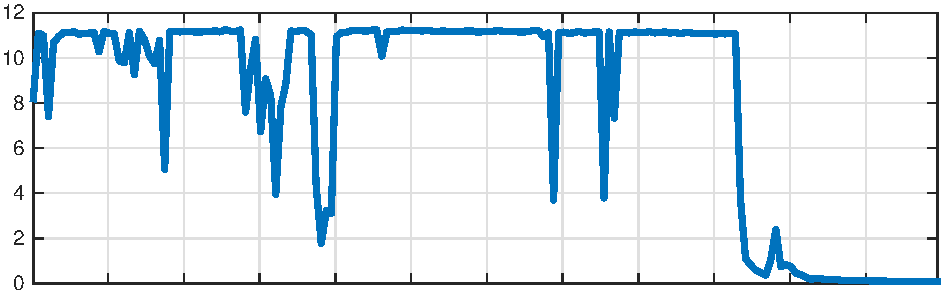
\includegraphics[valign=t,trim=0 0 5pt 0,angle=90,origin=tr,width=\sunintwidth,totalheight=\eventheight]{events/20141030-intensity.pdf}
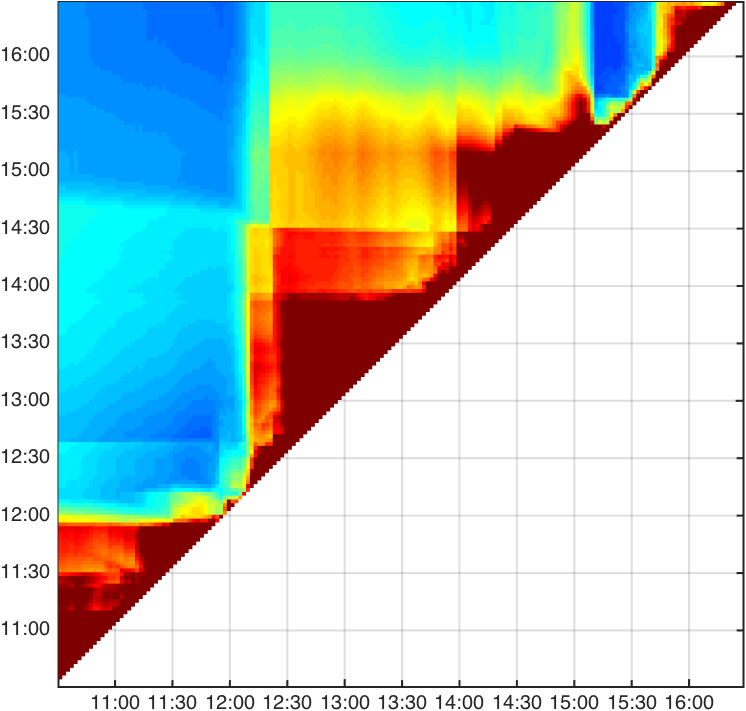
\includegraphics[valign=t,width=\eventswidth]{events/20141030-maxGain-local-events.png}
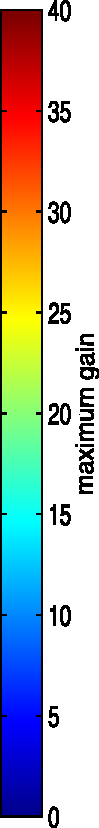
\includegraphics[valign=t,trim=2pt -8pt 0 5pt,width=\colorbarwidth,totalheight=\eventheight]{events/colorbar-40.pdf}
\end{minipage} \\*[1em]
\begin{minipage}[c]{\mylength}
\centering \scriptsize 2-NOV-14 \\
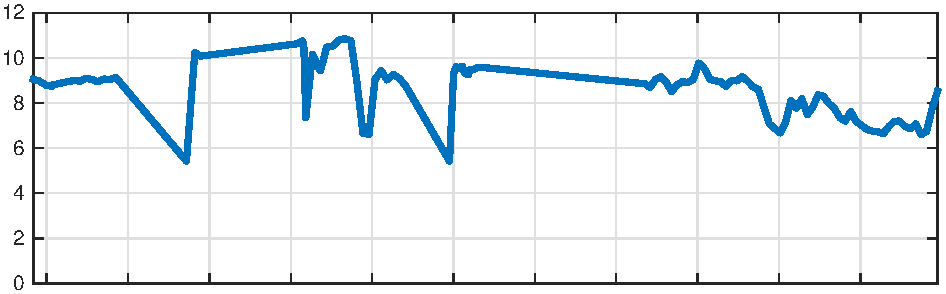
\includegraphics[valign=t,trim=0 0 5pt 0,angle=90,origin=tr,width=\sunintwidth,totalheight=\eventheight]{events/20141102-intensity.pdf}
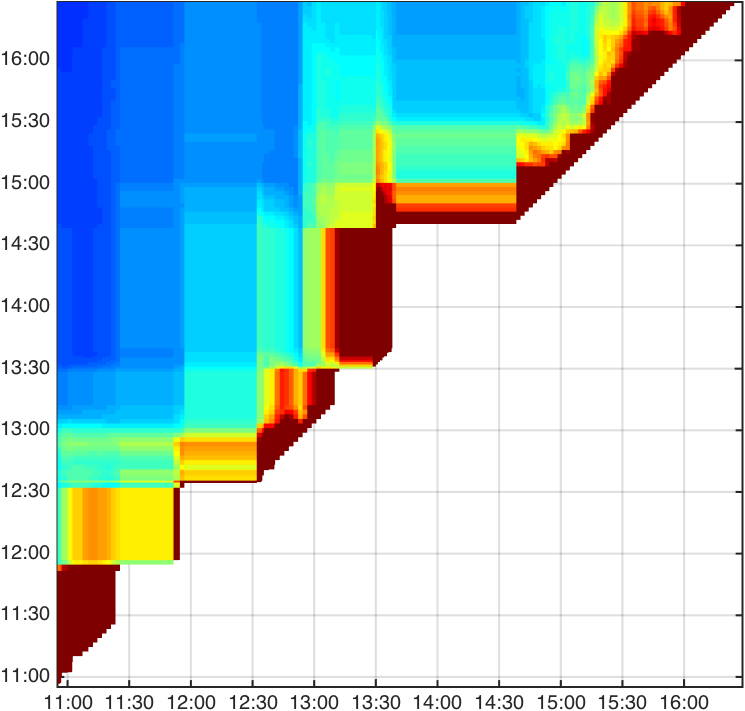
\includegraphics[valign=t,width=\eventswidth]{events/20141102-maxGain-local-events.png}
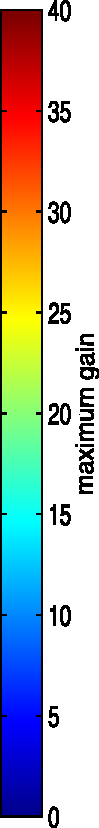
\includegraphics[valign=t,trim=2pt -8pt 0 5pt,width=\colorbarwidth,totalheight=\eventheight]{events/colorbar-40.pdf}
\end{minipage}
\begin{minipage}[c]{\mylength}
\centering \scriptsize 3-NOV-14 \\
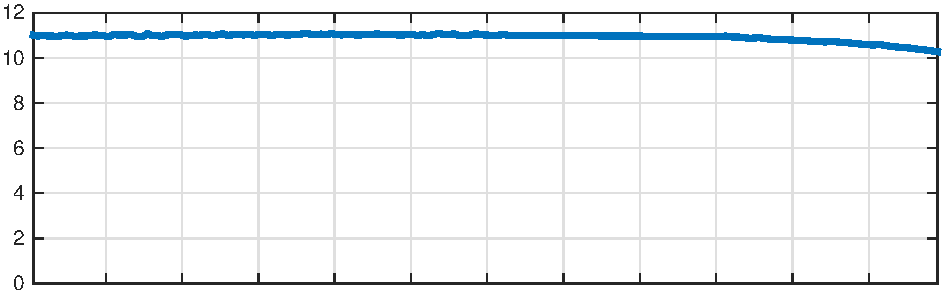
\includegraphics[valign=t,trim=0 0 5pt 0,angle=90,origin=tr,width=\sunintwidth,totalheight=\eventheight]{events/20141103-intensity.pdf}
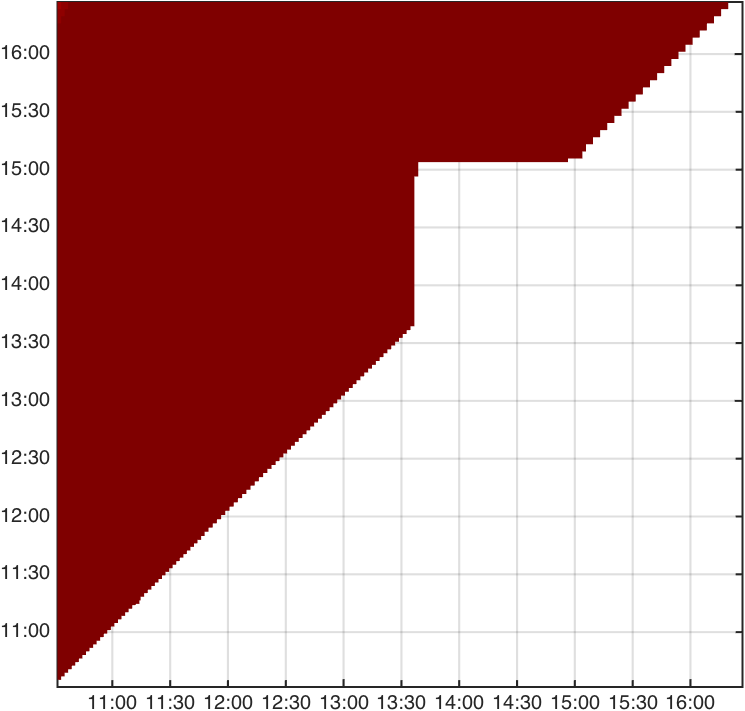
\includegraphics[valign=t,width=\eventswidth]{events/20141103-maxGain-local-events.png}
\includegraphics[valign=t,trim=2pt -8pt 0 5pt,width=\colorbarwidth,totalheight=\eventheight]{events/colorbar-40.pdf}
\end{minipage}
\begin{minipage}[c]{\mylength}
\centering \scriptsize 8-NOV-14 \\
\includegraphics[valign=t,trim=0 0 5pt 0,angle=90,origin=tr,width=\sunintwidth,totalheight=\eventheight]{events/20141108-intensity.pdf}
\includegraphics[valign=t,width=\eventswidth]{events/20141108-maxGain-local-events.png}
\includegraphics[valign=t,trim=2pt -8pt 0 5pt,width=\colorbarwidth,totalheight=\eventheight]{events/colorbar-40.pdf}
\end{minipage}  \\*[1em]
\begin{minipage}[c]{\mylength}
\centering \scriptsize 10-NOV-14 \\
\includegraphics[valign=t,trim=0 0 5pt 0,angle=90,origin=tr,width=\sunintwidth,totalheight=\eventheight]{events/20141110-intensity.pdf}
\includegraphics[valign=t,width=\eventswidth]{events/20141110-maxGain-local-events.png}
\includegraphics[valign=t,trim=2pt -8pt 0 5pt,width=\colorbarwidth,totalheight=\eventheight]{events/colorbar-40.pdf}
\end{minipage}
\begin{minipage}[c]{\mylength}
\centering \scriptsize 11-NOV-14 \\
\includegraphics[valign=t,trim=0 0 5pt 0,angle=90,origin=tr,width=\sunintwidth,totalheight=\eventheight]{events/20141111-intensity.pdf}
\includegraphics[valign=t,width=\eventswidth]{events/20141111-maxGain-local-events.png}
\includegraphics[valign=t,trim=2pt -8pt 0 5pt,width=\colorbarwidth,totalheight=\eventheight]{events/colorbar-40.pdf}
\end{minipage}
\begin{minipage}[c]{\mylength}
\centering \scriptsize 13-NOV-14 \\
\includegraphics[valign=t,trim=0 0 5pt 0,angle=90,origin=tr,width=\sunintwidth,totalheight=\eventheight]{events/20141113-intensity.pdf}
\includegraphics[valign=t,width=\eventswidth]{events/20141113-maxGain-local-events.png}
\includegraphics[valign=t,trim=2pt -8pt 0 5pt,width=\colorbarwidth,totalheight=\eventheight]{events/colorbar-40.pdf}
\end{minipage} \\*[1em]
\begin{minipage}[c]{\mylength}
\centering \scriptsize 14-NOV-14 \\
\includegraphics[valign=t,trim=0 0 5pt 0,angle=90,origin=tr,width=\sunintwidth,totalheight=\eventheight]{events/20141114-intensity.pdf}
\includegraphics[valign=t,width=\eventswidth]{events/20141114-maxGain-local-events.png}
\includegraphics[valign=t,trim=2pt -8pt 0 5pt,width=\colorbarwidth,totalheight=\eventheight]{events/colorbar-40.pdf}
\end{minipage}
\vspace{1em}
\caption{Fine-grained analysis of the expected uncertainty of outdoor PS (additional results for fig. 5 in the paper). Blank spaces above the diagonal indicate time intervals with missing data. Continued from fig.~\ref{fig:fig-5-1}.}
\label{fig:fig-5-2}
\end{figure*}

\begin{figure*}
\centering
\includegraphics[width=\mylength]{dist/20130711-maxGain-local-relativePerf}
\includegraphics[width=\mylength]{dist/20130816-maxGain-local-relativePerf}
\includegraphics[width=\mylength]{dist/20130823-maxGain-local-relativePerf} \\
\parbox{\mylength}{\centering 07-JUL-13}
\parbox{\mylength}{\centering 16-AUG-13}
\parbox{\mylength}{\centering 23-AUG-13} \\*[1em]
\includegraphics[width=\mylength]{dist/20130824-maxGain-local-relativePerf}
\includegraphics[width=\mylength]{dist/20131106-maxGain-local-relativePerf}
\includegraphics[width=\mylength]{dist/20131111-maxGain-local-relativePerf} \\
\parbox{\mylength}{\centering 24-AUG-13}
\parbox{\mylength}{\centering 06-NOV-13}
\parbox{\mylength}{\centering 11-NOV-13} \\*[1em]
\includegraphics[width=\mylength]{dist/20131115-maxGain-local-relativePerf}
\includegraphics[width=\mylength]{dist/20131119-maxGain-local-relativePerf}
\includegraphics[width=\mylength]{dist/20141003-maxGain-local-relativePerf} \\
\parbox{\mylength}{\centering 15-NOV-13}
\parbox{\mylength}{\centering 19-NOV-13}
\parbox{\mylength}{\centering 03-OCT-14} \\*[1em]
\includegraphics[width=\mylength]{dist/20141006-maxGain-local-relativePerf}
\includegraphics[width=\mylength]{dist/20141011-maxGain-local-relativePerf}
\includegraphics[width=\mylength]{dist/20141020-maxGain-local-relativePerf} \\
\parbox{\mylength}{\centering 06-OCT-14}
\parbox{\mylength}{\centering 11-OCT-14}
\parbox{\mylength}{\centering 20-OCT-14} \\*[1em]
\caption{Distribution of noise gain ratio $r_t$ as a function of time interval duration (additional results for fig. 6 in the paper). Continued on fig.~\ref{fig:fig-6-2}.}
\label{fig:fig-6-1}
\end{figure*}

\begin{figure*}
\centering
\includegraphics[width=\mylength]{dist/20141021-maxGain-local-relativePerf}
\includegraphics[width=\mylength]{dist/20141022-maxGain-local-relativePerf}
\includegraphics[width=\mylength]{dist/20141030-maxGain-local-relativePerf} \\
\parbox{\mylength}{\centering 21-OCT-14}
\parbox{\mylength}{\centering 22-OCT-14}
\parbox{\mylength}{\centering 30-OCT-14} \\*[1em]
\includegraphics[width=\mylength]{dist/20141102-maxGain-local-relativePerf}
\includegraphics[width=\mylength]{dist/20141103-maxGain-local-relativePerf}
\includegraphics[width=\mylength]{dist/20141108-maxGain-local-relativePerf} \\
\parbox{\mylength}{\centering 02-NOV-14}
\parbox{\mylength}{\centering 03-NOV-14}
\parbox{\mylength}{\centering 08-NOV-14} \\*[1em]
\includegraphics[width=\mylength]{dist/20141110-maxGain-local-relativePerf}
\includegraphics[width=\mylength]{dist/20141111-maxGain-local-relativePerf} 
\includegraphics[width=\mylength]{dist/20141113-maxGain-local-relativePerf} \\
\parbox{\mylength}{\centering 10-NOV-14}
\parbox{\mylength}{\centering 11-NOV-14}
\parbox{\mylength}{\centering 13-NOV-14} \\*[1em]
\includegraphics[width=\mylength]{dist/20141114-maxGain-local-relativePerf} \\
\parbox{\mylength}{\centering 14-NOV-14}
\caption{Distribution of noise gain ratio $r_t$ as a function of time interval duration (additional results for fig. 6 in the paper). Continued from fig.~\ref{fig:fig-6-1}.}
\label{fig:fig-6-2}
\end{figure*}


\FloatBarrier
\begin{table}
\centering
\begin{tabular}{|c|c|c|} \hline
 & \multicolumn{2}{|c|}{Beginning time} \\ \hline
Interval & 12h & 13h30 \\ \hline \hline
1h & 7 & 8 \\ \hline
2h & 15 & 15 \\ \hline
3h & 22 & 23 \\ \hline
4h & 30 &  \\ \hline
5h & 37 &  \\ \hline
6h & 39 &  \\ \hline
\end{tabular}
\vspace{.5em}
\caption{Quantity of input images used for each interval in fig.~\ref{fig:luxrender-results}.}
\label{tab:luxrender-qty-input}
\end{table}


\definecolor{Gray}{gray}{0.8}
\begin{figure*}
\centering
\begin{tabular}{ccccc}
\colorbox{Gray}{\includegraphics[height=3cm]{recons/bunny-input-01.png}} &
\colorbox{Gray}{\includegraphics[height=3cm]{recons/bunny-input-02.png}} &
\colorbox{Gray}{\includegraphics[height=3cm]{recons/bunny-input-03.png}} &
\colorbox{Gray}{\includegraphics[height=3cm]{recons/bunny-input-04.png}} &
\colorbox{Gray}{\includegraphics[height=3cm]{recons/bunny-input-05.png} }\\
\colorbox{Gray}{\includegraphics[height=3cm]{recons/owl-input-01.png}} &
\colorbox{Gray}{\includegraphics[height=3cm]{recons/owl-input-02.png}} &
\colorbox{Gray}{\includegraphics[height=3cm]{recons/owl-input-03.png}} &
\colorbox{Gray}{\includegraphics[height=3cm]{recons/owl-input-04.png}} &
\colorbox{Gray}{\includegraphics[height=3cm]{recons/owl-input-05.png}} \\
12:00 & 13:30 & 14:30 & 15:30 & 16:30
\end{tabular}
\vspace{.5em}
\caption{\small Example of input images used for reconstruction. These images are obtained using the physically-based rendering engine LuxRender. For each image, one environment map from the database was used as the sole light source. The ground was modeled with a constant albedo approximating the asphalt, $\rho = 0.15$. The rendering engine realistically simulates complex lighting effects such as cast shadows and inter-reflections (such as the neck of the bunny or below the eyebrows of the owl). }
\label{fig:luxrender-input}
\end{figure*}


\begin{figure*}
\centering
\footnotesize
\begin{tabular}{cc}
\hspace{0.1cm}\includegraphics[height=5.35cm,width=0.58\textwidth]{recons/owl-left.pdf} & 
\includegraphics[height=5.35cm,width=0.38\textwidth]{recons/owl-right.pdf} \\
\includegraphics[height=5.35cm,width=0.58\textwidth]{recons/bunny-left.pdf} & 
\includegraphics[height=5.35cm,width=0.38\textwidth]{recons/bunny-right.pdf} \\
(a) Intervals starting at 12:00 on 06-NOV-13 & (b) Intervals starting at 13:30 on 06-NOV-13
\end{tabular}
\vspace{.5em}
\caption{\small Surface reconstruction errors as a function of interval duration and start times: (a) 12h00 and (b) 13h30 on 06-NOV-13 (see fig. 5-(d) and 7 of the paper). Experiments are performed on the images described in fig.~\ref{fig:luxrender-input}. The top row shows per-pixel angular error, color-coded according to the scale on the right. The bottom row shows a box-percentile plot of the errors, as explained in the paper. The red horizontal bars indicate the median, while the bottom (top) blue bars are the 25th (75th) percentiles. Note how, as captured in fig. 5 and 7 of the paper, normal estimation can yield very similar results in 3h over that day using only 3 hours of data (a), and even from just one hour (b). The discrepancies between these results and fig. 5 of the paper are explained by cast shadows and inter-reflections (mainly present on bunny's neck and between its legs and on the corners of the eyes of the owl) which are not modeled by the reconstruction algorithm.}
\label{fig:luxrender-results}
\end{figure*}



% Definitions 
% \input{definitions}


% {\small
% \bibliographystyle{ieee}
% \bibliography{main}
% }

